\documentclass[border=1cm]{standalone}

%\usepackage{tikz}
\usepackage{amsmath}
\usepackage{pgfplots}
\usepackage{gensymb}
\usepackage{pgfplots}
\usepackage{pgfplotstable}
\usepackage{bm}
\usepackage{amssymb}
\usepackage[siunitx]{circuitikz}
\usetikzlibrary{shapes, arrows.meta, positioning, decorations.pathmorphing, math, calc, fit, chains, matrix, decorations.pathreplacing, decorations.markings}

\pgfplotsset{compat=1.15}
\newcommand{\mosfet}[1]{%
    \draw (#1.B) -- ($(#1.B)+(0.3,0)$);%
    \draw ($(#1.B)+(0.3,0.3)$) -- ($(#1.B)+(0.3,-0.3)$);%
    \draw ($(#1.B)+(0.4,0.3)$) -- ($(#1.B)+(0.4,-0.3)$);%
    \draw ($(#1.B)+(0.5,0.4)$) -- ($(#1.B)+(0.5,-0.4)$);%
    \draw ($(#1.B)+(0.5,0.3)$) -| (#1.D);
    \draw ($(#1.B)+(0.5,-0.3)$) -| (#1.S);
}

\begin{document}

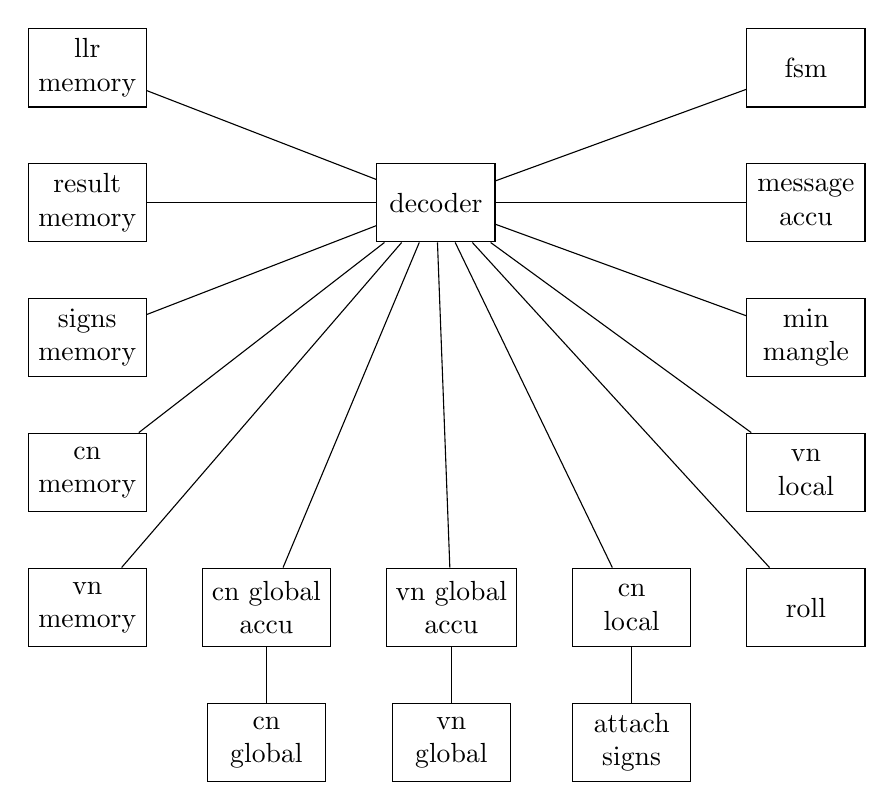
\begin{tikzpicture}[
    elem/.style={draw,rectangle,node distance=0.7cm,align=center,minimum width=1.5cm, minimum height=1cm},
    circ/.style={draw,circle,node distance=1cm,align=center,minimum width=1.5cm, minimum height=1cm},
    branch/.style={fill,shape=circle,minimum size=3pt,inner sep=0pt}]
    \node (llr) [elem] {llr\\memory};
    \node (res) [elem,below=of llr] {result\\memory};
    \node (sig) [elem,below=of res] {signs\\memory};
    \node (cnm) [elem,below=of sig] {cn\\memory};
    \node (vnm) [elem,below=of cnm] {vn\\memory};
    \node (vna) [elem,right=of vnm] {cn global\\accu};
    \node (vng) [elem,below=of vna] {cn\\global};
    \node (cna) [elem,right=of vna] {vn global\\accu};
    \node (cng) [elem,below=of cna] {vn\\global};
    \node (cnl) [elem,right=of cna] {cn\\local};
    \node (att) [elem,below=of cnl] {attach\\signs};
    \node (rol) [elem,right=of cnl] {roll};
    \node (vnl) [elem,above=of rol] {vn\\local};
    \node (mim) [elem,above=of vnl] {min\\mangle};
    \node (mea) [elem,above=of mim] {message\\accu};
    \node (fsm) [elem,above=of mea] {fsm};
    \node (tmp) [elem,right=of res,opacity=0.0] {};
    \node (dec) [elem,right=of tmp] {decoder};
    \draw (llr) -- (dec);
    \draw (res) -- (dec);
    \draw (sig) -- (dec);
    \draw (cnm) -- (dec);
    \draw (vnm) -- (dec);
    \draw (vna) -- (dec);
    \draw (vng) -- (vna);
    \draw (cna) -- (dec);
    \draw (cng) -- (cna);
    \draw (cnl) -- (dec);
    \draw (att) -- (cnl);
    \draw (rol) -- (dec);
    \draw (vnl) -- (dec);
    \draw (mim) -- (dec);
    \draw (mea) -- (dec);
    \draw (fsm) -- (dec);
\end{tikzpicture}
    
\end{document}
